%ATLAS weak mixing angle~\cite{Aad:2015uau}

In the electroweak theory the weak mixing angle $\theta_W$ is a free
parameter indicating the degree of mixing between $SU(2)_L$ and
$U(1)_Y$ neutral gauge bosons upon electroweak symmetry breaking to
obtain the physical neutral gauge bosons $\gamma$ and $\Zzero$.
Experimentally, it is typically measured as $\sin^2\theta_W$ via
angular distributions in fermion pair production; it has been most
precisely measured at the LEP 1 and SLD experiments via fermion pair
production at the $\Zzero$ pole, yielding a combined value of
$0.23153\pm0.00016$~\cite{ALEPH:2005ab}. In the standard model it is
related to the gauge boson masses at tree level by $1-m_W^2/m_Z^2$ and
modified by higher-order loop corrections, including contributions
from Higgs boson loops; the effective angle measured upon introducing
loop corrections is denoted as $\sin^2\theta^{eff}_{W}$. The recent
high-precision Higgs boson mass measurement at the LHC combined with
other electroweak measurements can be used to predict a value for
$\sin^2\theta^{eff}_{W}$ of $0.23149 \pm 0.00007$~\cite{Baak:2014ora},
motivating an improvement upon the direct experimental measurement
precision by a factor of two or more at the LHC to constrain the
electroweak theory further.

At a hadron collider, fermion pair production at and around the $\Zzero$
pole is measured in the process
$q\bar{q}\rightarrow \gamma^*/Z \rightarrow \ell^+\ell^-$, where the
differential scattering cross section is characterized by
$d^3\sigma/dm \ dy \ d\cos\theta = A(m,y)(1+\cos^2\theta) +
B(m,y)\cos\theta$, where $m$ is the final state lepton pair mass, $y$
is the lepton pair rapidity, and $\cos\theta$ is the polar angle of
the positive lepton with respect to the quark direction. A
non-vanishing forward-backward asymmetry in this angle, $A_{FB}(m,y) =
3B(m,y)/8A(m,y)$, arises from interference between vector and
axial-vector currents; the portion of $A_{FB}(m,y)$ corresponding to
self-interference of the $\Zzero$ boson currents is directly sensitive to
$\sin^2\theta^{eff}_{W}$.

In hadron collisions, the quark direction is ambiguous, as it may
originate from either incoming hadron and have unknown transverse
momentum. The impact of quark transverse momentum on the
forward-backward assignment is minimized by defining the quark
direction to be the difference between the forward-going and
backward-going hadron momentum vectors in the lepton pair rest frame,
as originally suggested by Collins and Soper~\cite{Collins:1977iv};
this angle is typically denoted as $\cos\theta^*$. In proton-proton
collisions, the ambiguity due to quark origination is an irreducible
dilution in $A_{FB}$ which is strongest at low $|y|$ and decreasing at
higher $|y|$ where valence quark/sea anti-quark annihilation is
predominant; measurements of $A_{FB}(m,y)$ at high-$|y|$ are therefore
intrinsically more sensitive to the undiluted value and have smaller
theory uncertainties related to PDFs.  In proton--anti-proton
collisions, valence quark/valence anti-quark annihilation
predominates, and so dilution and its associated uncertainties are
vastly reduced, making the Tevatron experimental
measurements~\cite{Aaltonen:2016nuy,Aaltonen:2014loa,Abazov:2014jti} a
competitive alternative to the LHC for current data samples. Three LHC
experiments have measured $\sin^2\theta^{eff}_{W}$: an initial
exploratory measurement by CMS at 7 TeV~\cite{Chatrchyan:2011ya}, a
measurement by ATLAS with all 7 TeV data~\cite{Aad:2015uau}, and a
measurement by LHCb~\cite{Alves:2008zz,Aaij:2014jba} with all 7 and 8
TeV data~\cite{Aaij:2015lka}.

The ATLAS measurement was performed with three different samples: muon
pairs with $\pt > 20$ GeV and $|\eta| < 2.4$; electron pairs with $E_T
> 25$ GeV and $|\eta| < 2.47$; and electron pairs with $E_T > 25$ GeV
where one has $|\eta| < 2.47$ and the other has $2.5 < |\eta| < 4.9$.
In the last case the forward electron is identified with calorimeters
alone, still the resulting pairs have a signal purity at the
$\Zzero$ pole of 95\%.  The data in each sample $i$ are binned in mass, and
the raw measured angular asymmetry in that region of phase space,
$A^{\rm meas}_{FB, i}(m)$, is computed from counting forward
($\cos\theta^* > 0$) and backward ($\cos\theta^* < 0$) candidates
after background subtraction.  Each $A_{FB,i}$ is used to extract
$\sin^2\theta^{eff}_{W}$ via a binned $\chi^2$ fit of
LO \texttt{PYTHIA} templates of different mixing angle values to the
data.  Figure~\ref{fig:ss-precision-afb-atlas-cf} shows the
$\cos\theta^*$ distribution for selected central-forward electron
pairs; an asymmetry between forward and backward angles is visually
evident.  Figure~\ref{fig:ss-precision-afb-atlas-cf} also show the
resulting $A^{\rm meas}_{FB}(m)$, alongside the best-fit predictions
from LO \texttt{PYTHIA} and NLO \texttt{POWHEG}.  The three samples
give consistent values for $\sin^2\theta^{eff}_{W}$ and are combined
to give a value of $0.2308 \pm 0.0005\textrm{(stat.)} \pm
0.0006\textrm{(syst.)} \pm 0.0009\textrm{(PDF)}$, where the last term
denotes the leading uncertainty in $\sin^2\theta^{eff}_{W}$ from
uncertainties in specially prepared LO PDFs consistent with the LO
PYTHIA template generation and 7 TeV ATLAS $W$ and $\Zzero$ data
(ATLAS-epWZ12 LO)~\cite{Aad:2011dm}.  A general feature of precision
electroweak measurements at the LHC is the predominance of PDF
uncertainties, requiring simultaneous PDF measurement with the
parameter of interest to obtain the best precision.  Other leading
systematic uncertainties are the lepton energy scale and MC template
statistics, which will improve with larger data sets.

The LHCb measurement employs a very similar technique.  They select
muon pairs with $\pt > 20$ GeV, $60 < m_{\mu\mu} < 160$ GeV, and $2.0 <
|\eta| < 4.5$, with a signal mass resolution and purity similar to
ATLAS but in a more forward, and therefore more sensitive, $\Zzero$
production region.  LHCb operational instantaneous luminosity is
limited to the range $2-4\times
10^{32}\textrm{cm}^{-2}\textrm{s}^{-1}$, however, so the sample size
is limited to $1\;\fb^{-1}$ at 7~TeV and $2\;\fb^{-1}$
at 8 TeV.  The data are binned in mass and $A_{FB}(m)$ is computed for
their acceptance, and then subsequently unfolded to account for mass
resolution effects. Figure~\ref{fig:ss-precision-afb-lhcb} shows the
unfolded $A_{FB}$ distribution at 8 TeV compared with NLO predictions
from \texttt{POWHEG-BOX}.  The unfolded $A_{FB}(m)$ distribution is
used to extract $\sin^2\theta^{eff}_{W}$ via a $\chi^2$ fit
of \texttt{POWHEG-BOX} templates of different mixing angle values to
the data.  They measure $\sin^2\theta^{eff}_{W} = 0.23142 \pm
0.00073 \textrm{(stat.)} \pm 0.00052 \textrm{(syst.)} \pm
0.00056 \textrm{(th.)}$, where the last term denotes uncertainties
from theoretical modelling ingredients, predominantly PDFs.  The PDF
uncertainties are evaluated from QCD+QED NLO NNPDF
2.3~\cite{Ball:2013hta,Ball:2012cx}, which, similar to the ATLAS PDF,
includes 7 TeV electroweak production data from the LHC.  In contrast
to the ATLAS result, the LHCb measurement statistically limited, but
has 30\% smaller theoretical uncertainties due to better understood
PDF uncertainties in the more forward production region.

A comparison of experimental measurements of
$\sin^2\theta^{eff}_{W}$~\cite{Aaltonen:2016nuy} is shown in
Figure~\ref{fig:ss-precision-summary-sin2thetaw}.  The best single
measurements from the Tevatron are more than twice as precise as the
best measurements from the LHC, and the separate $A^{0,b}_{FB}$ and
$A_{l}$ results from $e^+e^-$ collisions are more than four times as
precise.  There are reasonable prospects for the LHC experiments
eventually surpassing these: ATLAS and CMS are expected to have
superior statistical uncertainties by the end of Run 2, and all of the
systematic and PDF uncertainties are expected to improve as well with
larger electroweak data samples.

%CMS Drell--Yan AFB 7 \TeV~\cite{Chatrchyan:2012dc}
%CMS Drell--Yan AFB 8 \TeV (CMS-PAS-SMP-14-004, to be published)
\begin{figure}[p]
    \centering
    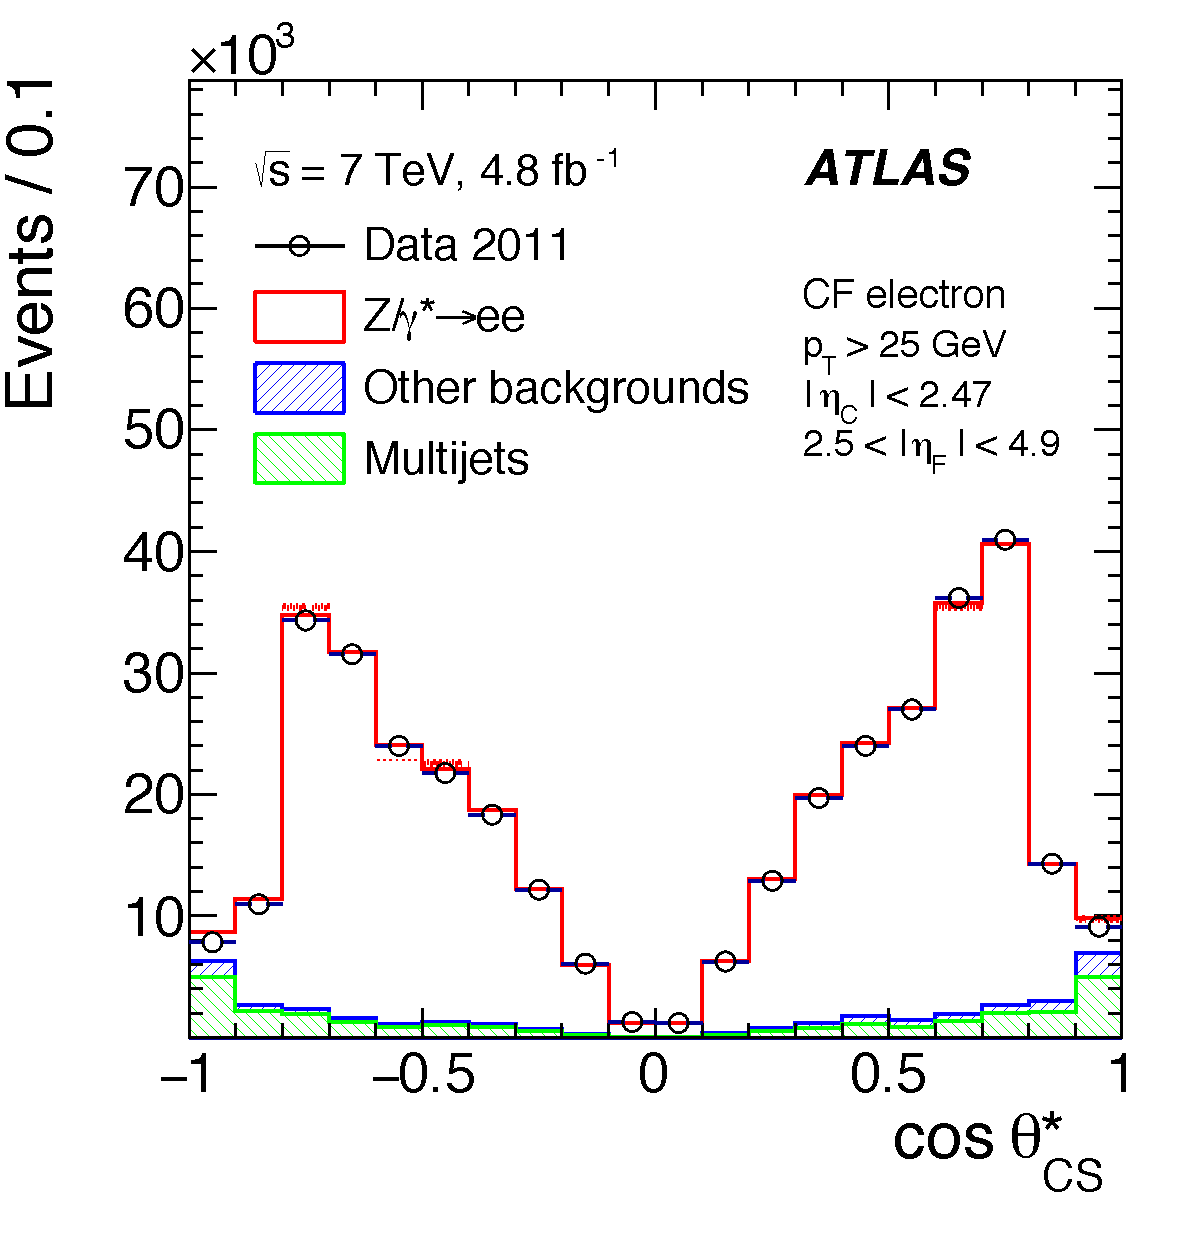
\includegraphics[width=0.45\textwidth]{figures/ss-precision-afb-atlas-cf-ct.pdf}
    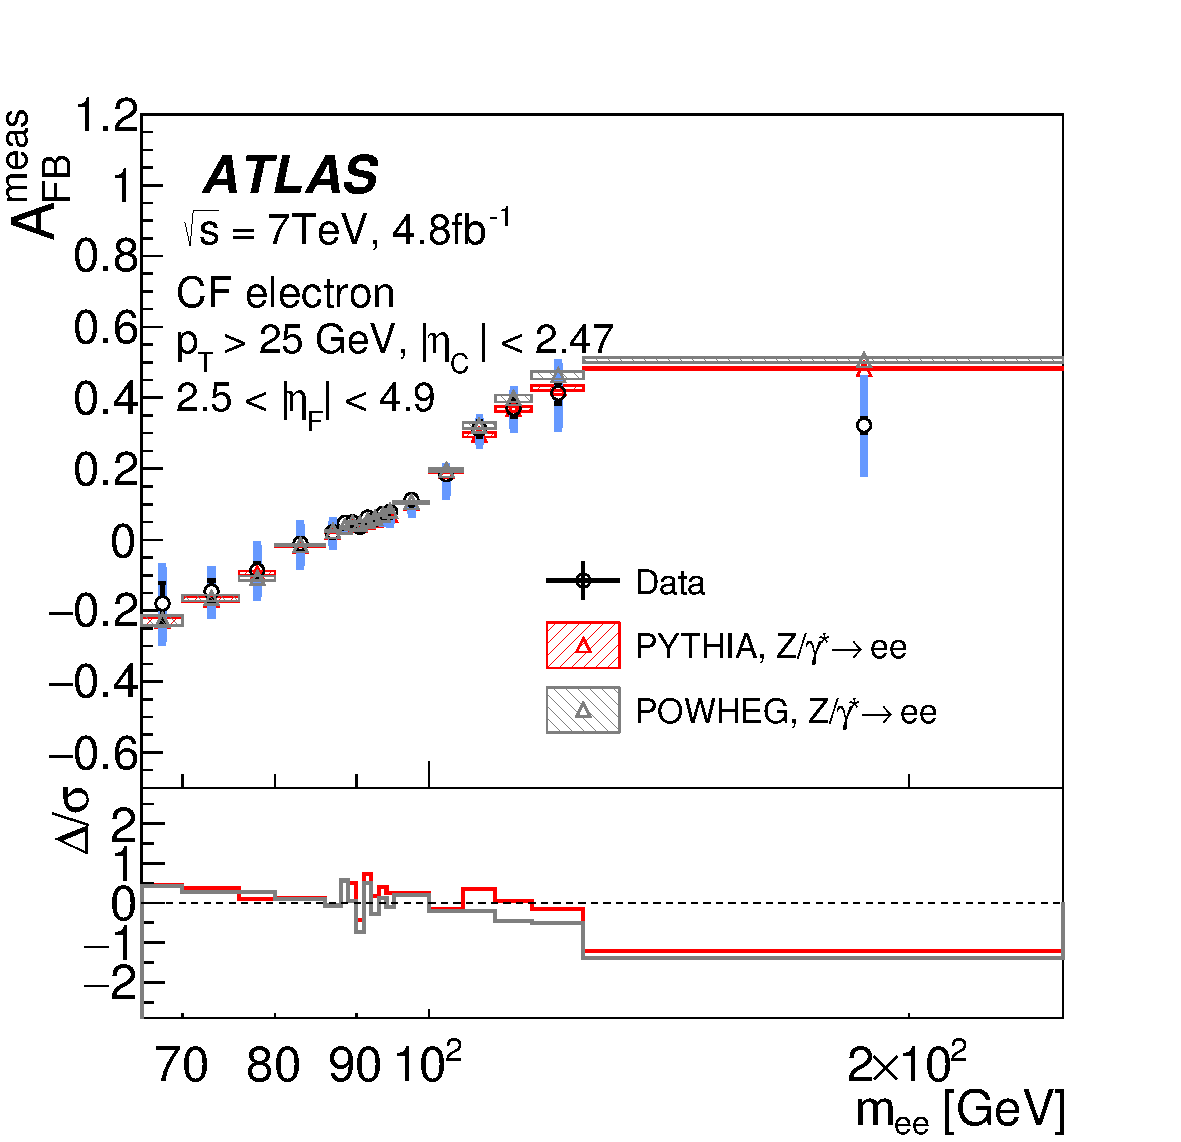
\includegraphics[width=0.45\textwidth]{figures/ss-precision-afb-atlas-cf-afb.pdf}
    \caption{
    From the ATLAS analysis of the full 7 TeV dataset~\cite{Aad:2015uau} on the left: The $\cos\theta^*$ distribution for selected central-forward electron pairs, compared with MC predictions.
    Right: $A^{\rm meas}_{FB}(m)$ for central-forward electron pairs, compared with MC predictions using the best fit $\sin^2\theta^{eff}_{W}$.}
    \label{fig:ss-precision-afb-atlas-cf}
\end{figure}

\begin{figure}[p]
    \centering
    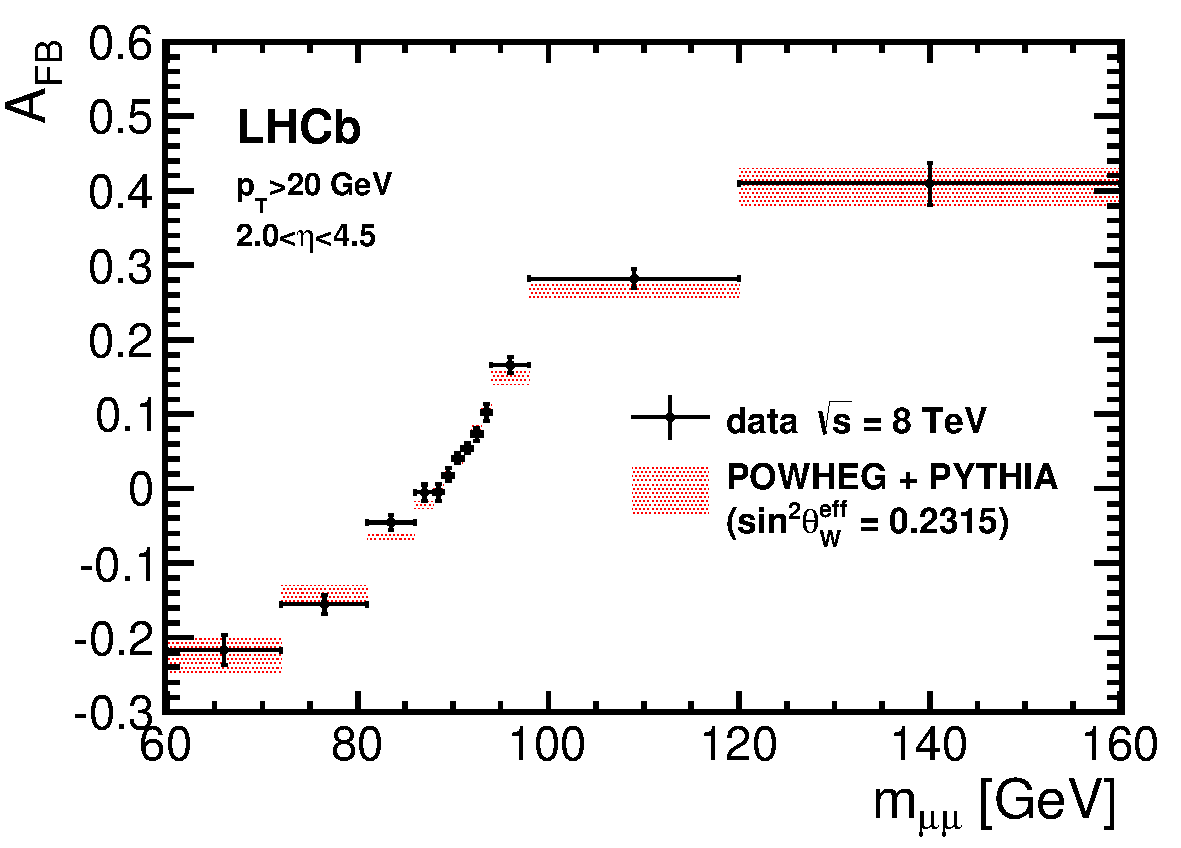
\includegraphics[height=0.3\textheight]{figures/ss-precision-afb-lhcb.pdf}
    \caption{The
unfolded $A_{FB}$ distribution from LHCb 8 TeV data , as a function of di-muon mass, compared with NLO predictions from \texttt{POWHEG-BOX}~\cite{Aaij:2015lka}.
    }
    \label{fig:ss-precision-afb-lhcb}
\end{figure}

\begin{figure}[p]
    \centering
    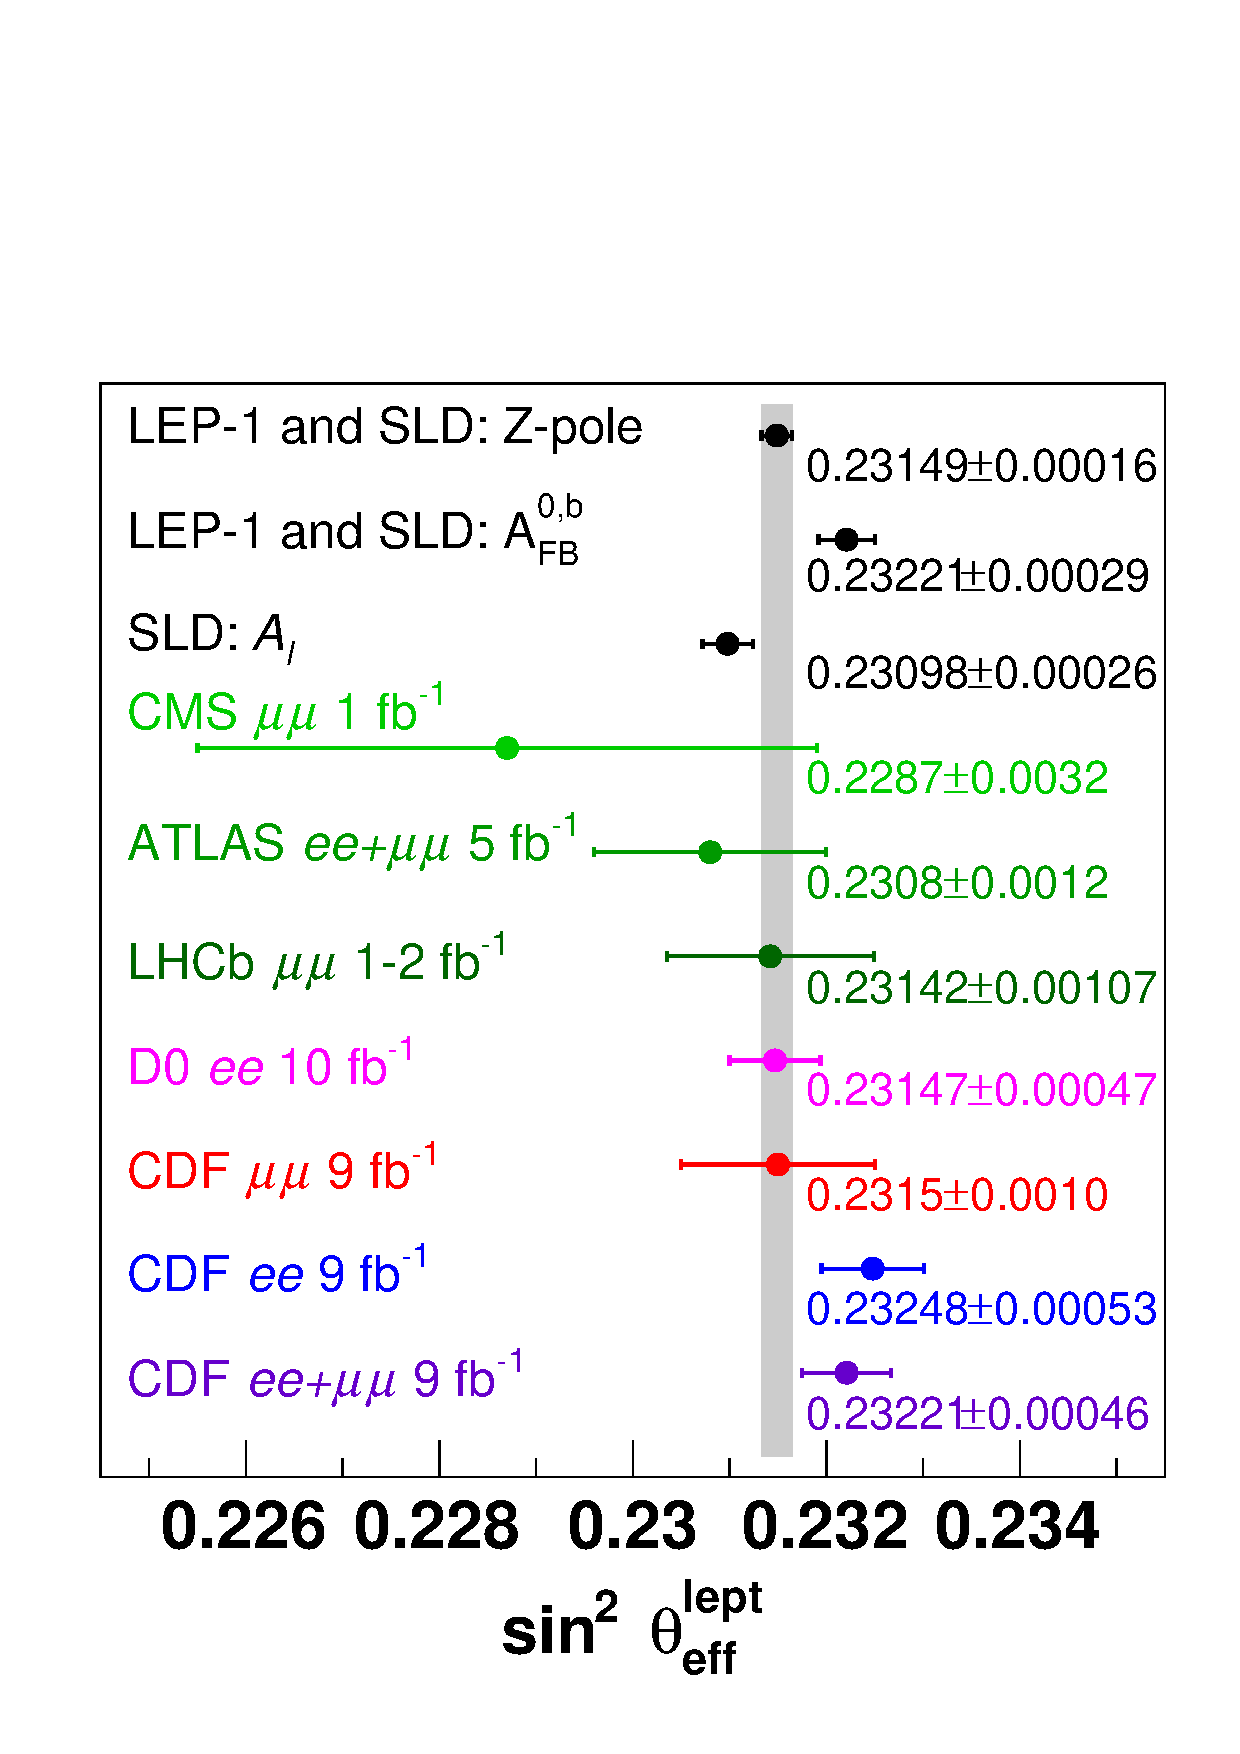
\includegraphics[height=0.3\textheight]{figures/ss-precision-summary-sin2thetaw.pdf}
    \caption{Comparison of experimental measurements of
$\sin^2\theta^{eff}_{W}$~\cite{Aaltonen:2016nuy}.}
    \label{fig:ss-precision-summary-sin2thetaw}
\end{figure}


